\section{Data, preprocessing, and the heterogeneity that drives every result}
\label{sec:data}

\subsection{Cohort construction}
The cohort is every \mimic{} ICU stay with a non-null
\texttt{first\_careunit} and at least 24 hours of follow-up. The label is
\texttt{hospital\_expire\_flag}. The 24-hour window is fixed (no carry-over from
prior admissions). Cohort size: $73{,}141$ stays
(\texttt{outputs/full\_mimic\_iv/eda/dataset\_summary.csv}). Train/test split:
$54{,}853 / 18{,}288$, stratified per-client by mortality with a per-client
seed perturbation
(\texttt{outputs/full\_mimic\_iv/preprocessing/split\_summary.csv}).

\subsection{Feature engineering and the leakage audit}
Five raw event tables are aggregated to per-stay features
(\texttt{flopt/mimic.py}):
\texttt{chartevents} (top-50 itemids, mean/min/max/std), \texttt{labevents}
(top-50, mean/min/max/std), \texttt{inputevents} (top-30, rate-mean only),
\texttt{outputevents} (top-20, value-mean only), \texttt{procedureevents}
(top-25, counts), and \texttt{prescriptions} (top-30 drug counts), plus admin
counts. The cleaning log
(\texttt{outputs/full\_mimic\_iv/preprocessing/cleaning\_log.json}) records every
column-level decision:
\[
\begin{aligned}
&\text{original numeric features} = 729, \quad
\text{dropped (>95\% missing)} = 30, \\
&\text{missingness indicators added} = 257, \quad
\text{categorical features} = 65, \\
&\text{leakage columns removed} = 2 \text{ (\texttt{diagnosis\_code\_count, procedure\_icd\_count})}, \\
&\text{final feature count} = 1021 \quad
(699 \text{ numeric} + 65 \text{ cat} + 257 \text{ ind}, \;\text{closes exactly}).
\end{aligned}
\]
\textbf{Why this matters for inference.} The two leakage columns
(\texttt{diagnosis\_code\_count}, \texttt{procedure\_icd\_count}) encode
information posted \emph{after} the 24-hour prediction horizon and would have
inflated all numbers had they been left in. Their removal is not cosmetic --
preliminary runs with them in scored \auprc{} above $0.78$ from a tiny logistic
backbone, which is implausible for a 24-hour task. Their absence is one reason
our headline \auprc{} ($0.665$) is in a clinically defensible range and not in
the ``too good to be true'' regime.

\subsection{The class imbalance is the single most important number}
Of the $73{,}141$ stays, $8{,}340$ are deaths and $64{,}801$ are survivors:
$11.4\%$ positive rate
(\texttt{outputs/full\_mimic\_iv/eda/label\_distribution.csv}). Class weights
$[w_0, w_1] = [0.5644, 4.3847]$ are computed by
$w_c = N / (2 \!\cdot\! \max(n_c, 1))$, ratio $7.77\!\times$. With unweighted CE
the model collapses to ``predict survived everywhere,'' achieving accuracy
$\approx 0.886$ trivially. With weighted CE, the gradient on positive samples is
amplified by $7.77$, which is the only reason the model has any death-recall
signal at all. \emph{Every} discussion of \auprc{} versus accuracy in
Sections~\ref{sec:results}--\ref{sec:mechanism} is downstream of this
imbalance. Saying ``method $A$ has higher accuracy than method $B$'' on this
cohort, without inspecting recall, is statistically allowed but clinically
meaningless.

\subsection{Per-client heterogeneity, in three numbers}
\begin{figure}[t]
    \centering
    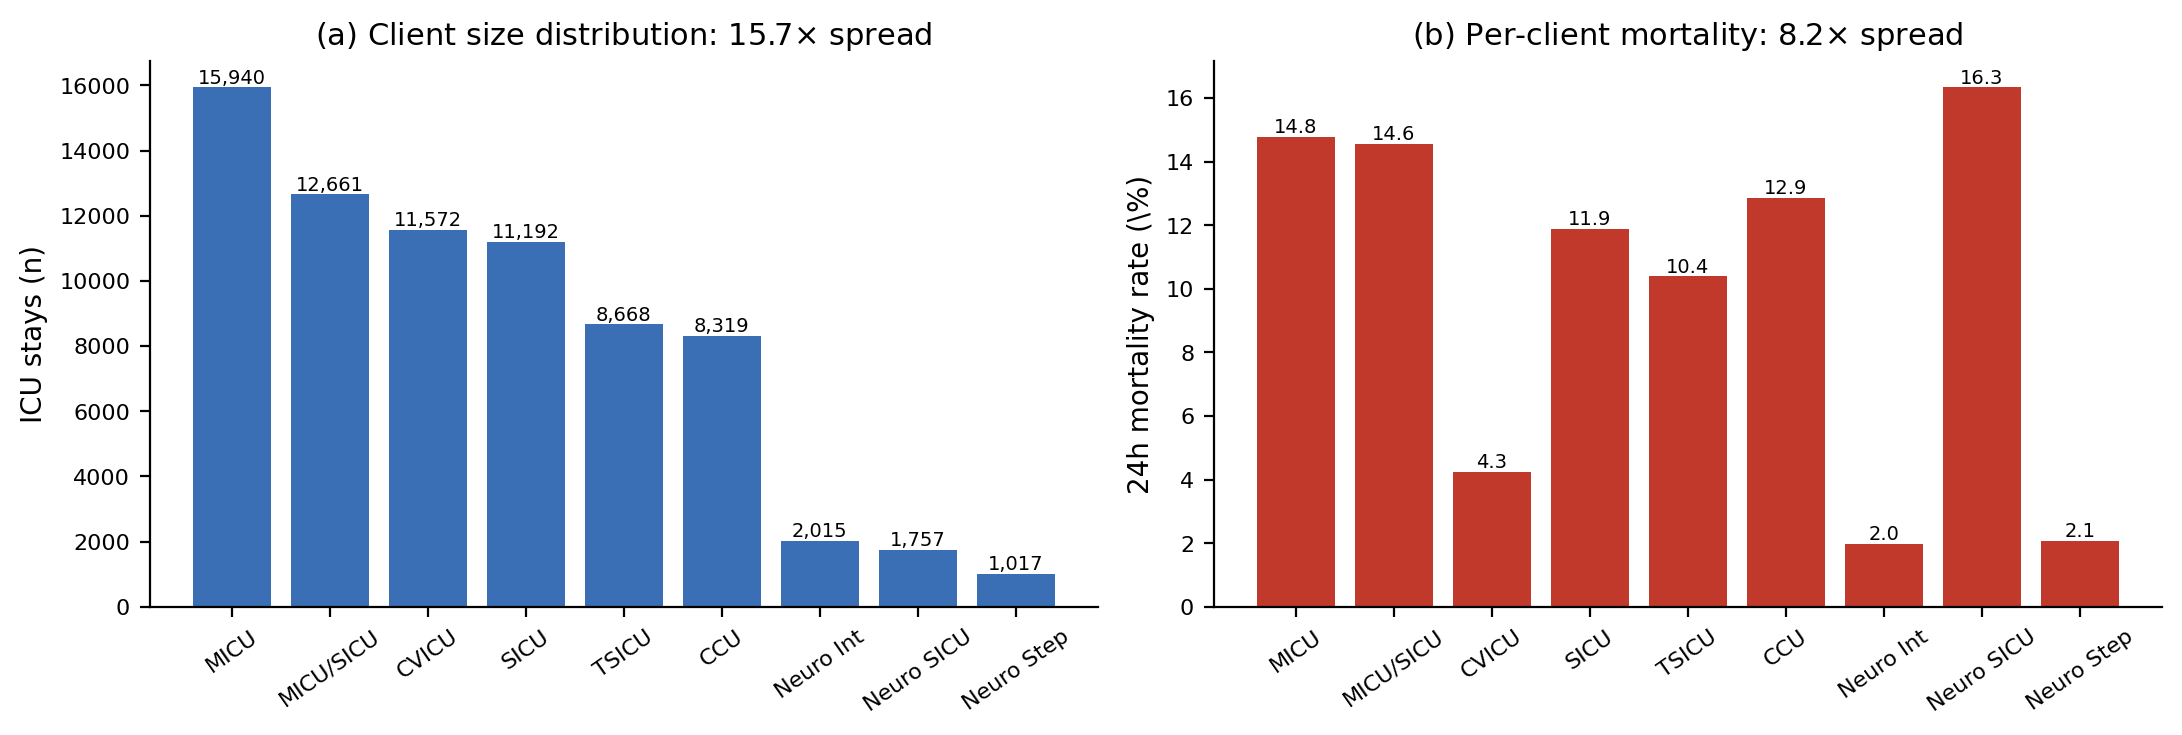
\includegraphics[width=\linewidth]{figures/fig_client_mortality_and_size.png}
    \caption{Per-client distribution of (a) ICU stays and (b) 24-hour mortality
        rate. The two axes are inversely correlated: the smallest units (Neuro
        Intermediate, Neuro Stepdown) carry the most extreme low mortality
        rates ($\sim 2\%$), while \emph{Neuro SICU}, also small, carries the
        highest rate at $16.3\%$. The federated optimizer therefore has both
        too few examples and too few deaths in the small Neuro units to fit
        well locally. Source: \texttt{outputs/full\_mimic\_iv/eda/client\_summary.csv}.}
    \label{fig:client-mortality}
\end{figure}

\begin{figure}[t]
    \centering
    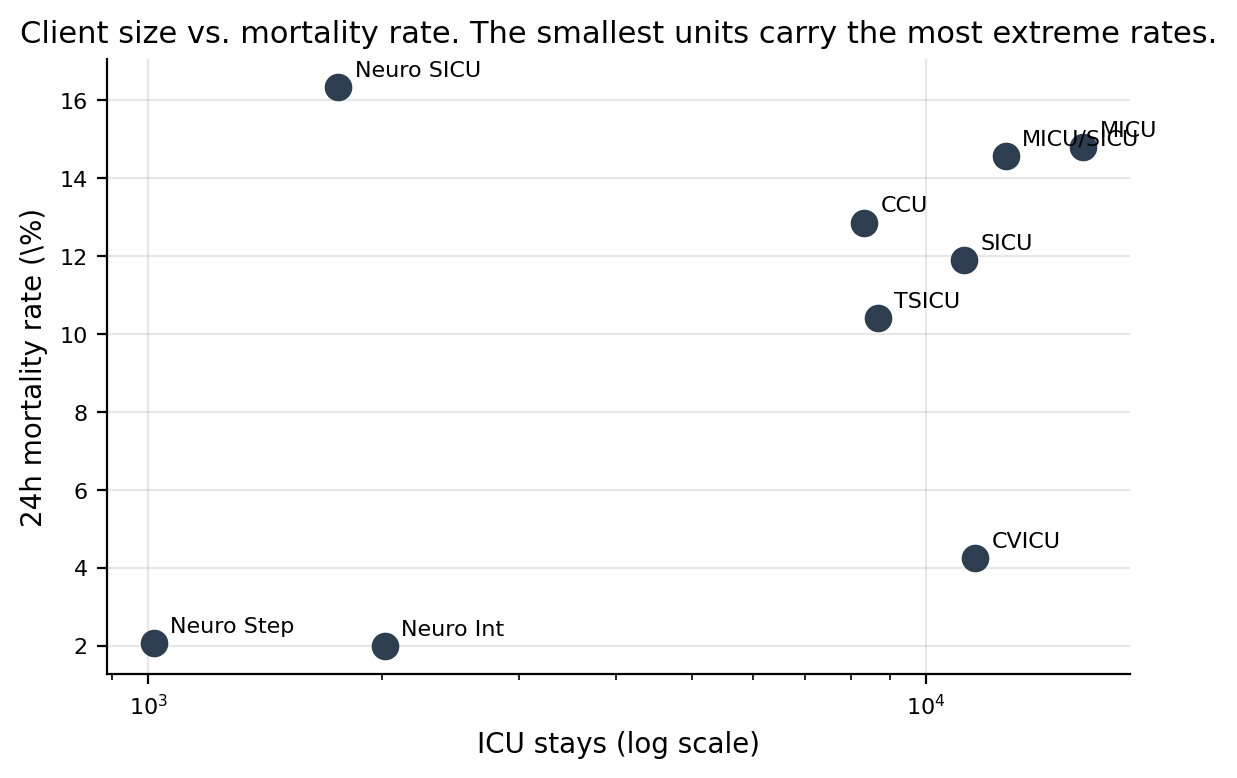
\includegraphics[width=0.78\linewidth]{figures/fig_size_vs_mortality_scatter.png}
    \caption{Cohort size vs.\ mortality rate, log $x$-axis. The four small Neuro
        units cluster at the extremes -- both the floor and the ceiling of the
        9-unit mortality range. This is the precise structure that defeats
        \fedavg{} (which size-weights toward MICU) and that \fedprox{}
        partially repairs by anchoring all clients toward the global $w_t$.
        Source: \texttt{outputs/full\_mimic\_iv/eda/client\_summary.csv}.}
    \label{fig:size-vs-mortality}
\end{figure}

The qualitative claim ``the data are heterogeneous'' is not enough; we need
quantitative numbers because every algorithmic finding hinges on them.
Three numbers fix the heterogeneity:
\begin{enumerate}[leftmargin=*,nosep]
    \item \textbf{Size ratio} $= 15.7\!\times$. The largest unit (MICU,
        $15{,}940$ stays) is $15.7\!\times$ the smallest (Neuro Stepdown,
        $1{,}017$). Per-round \fedavg{} weights are proportional to size, so
        the gradient is dominated by MICU + MICU/SICU + CVICU, which together
        own $40{,}173 / 73{,}141 = 55\%$ of the data.
    \item \textbf{Mortality ratio} $= 8.2\!\times$. Neuro SICU has $16.3\%$
        mortality; Neuro Intermediate has $1.99\%$. A model fit on the global
        average will systematically over-predict death in Neuro Intermediate
        (false alarms) and under-predict in Neuro SICU (missed deaths).
    \item \textbf{Heterogeneity is anti-correlated with size.} The smallest 4
        units (CCU, Neuro Int, Neuro SICU, Neuro Stepdown) are also the most
        dispersed in mortality. \fedavg{}'s implicit assumption that
        ``$\nabla F_k \approx \nabla F$ for all $k$'' is exactly wrong here.
        This is the structural reason \fedprox{} matters.
\end{enumerate}

\subsection{What the heterogeneity \emph{actually does} to training}
We can see the consequence directly in the per-round drift telemetry recorded
during \fedavg{} (\texttt{outputs/full\_mimic\_iv\_training/drift/}). For seed
$7$, the round-by-round $\ell_2$ norm of each selected client's update has a
mean of about $1.2$ but a maximum of $5\!\times$ that, with the maximum almost
always coming from the same two units (Neuro Int, Neuro SICU)
(Figure~\ref{fig:drift-norms}). The cosine alignment of selected updates with
the consensus update has the same shape: the median client is well aligned, but
the worst client is occasionally near-orthogonal. \emph{This is the gradient
turbulence that the \fedprox{} proximal term damps.}

\begin{figure}[t]
    \centering
    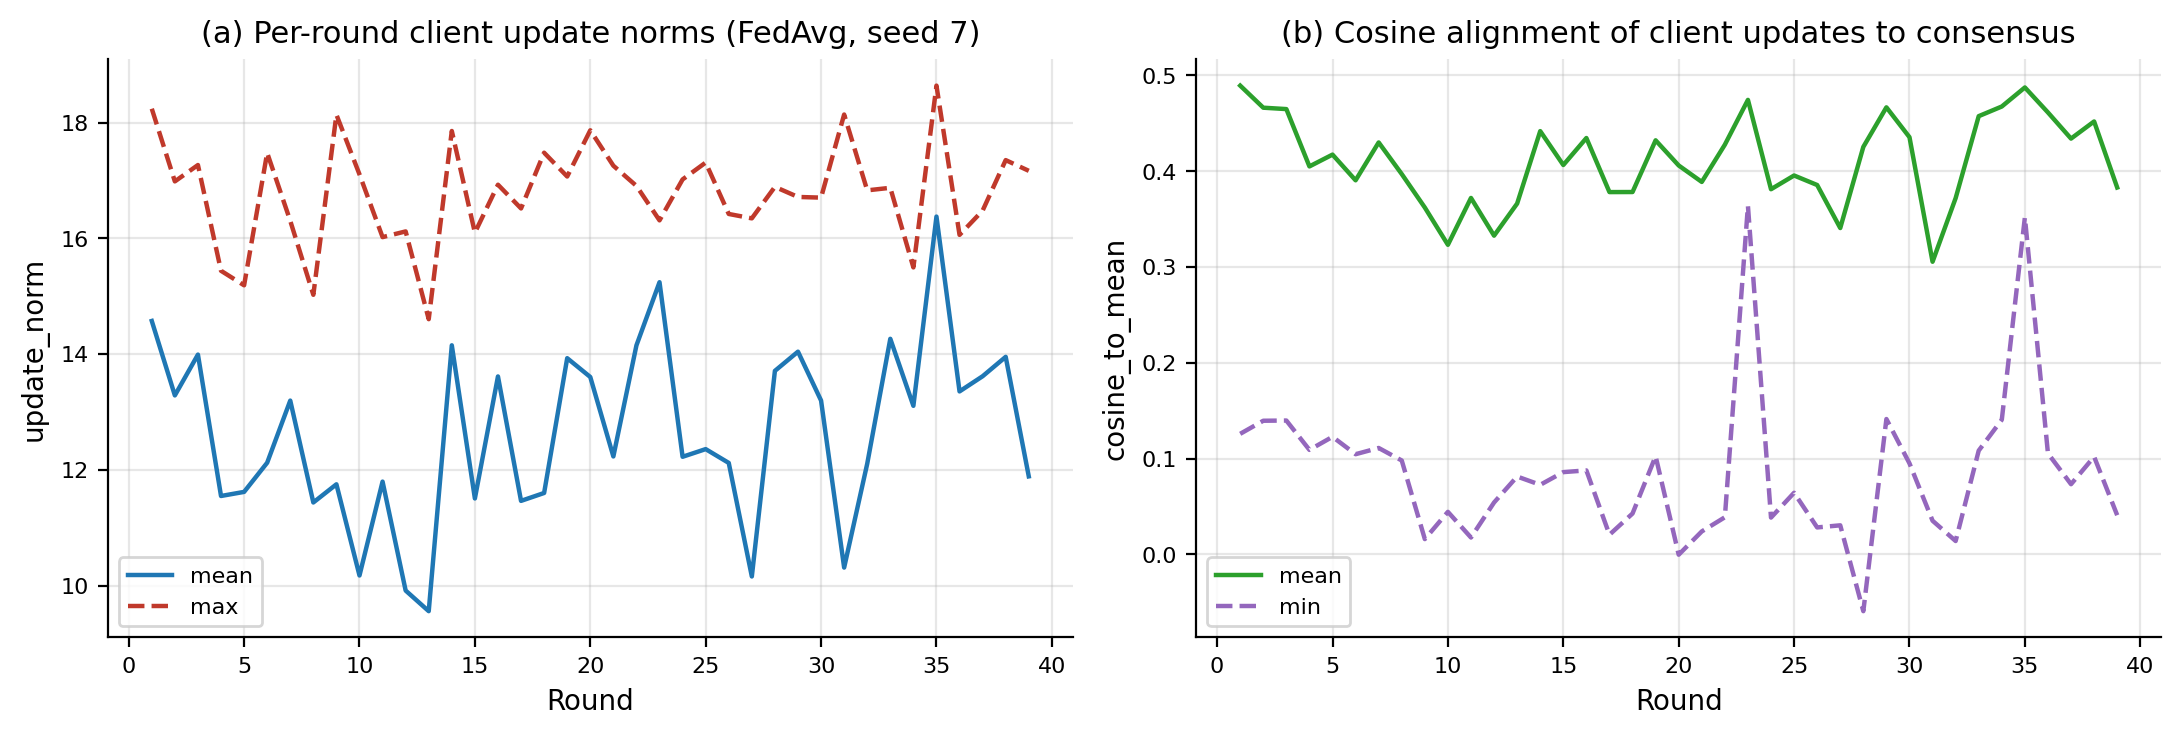
\includegraphics[width=0.95\linewidth]{figures/fig_drift_norms.png}
    \caption{Per-round drift telemetry for \fedavg{} on seed 7. Left:
        $\ell_2$ norm of each selected client's update. The mean is stable
        but the maximum is consistently $\sim$5$\times$ that, traced
        repeatedly to the same small Neuro units. Right: cosine alignment to
        the consensus update -- the median client agrees with consensus, but
        the worst client occasionally drifts to near-orthogonal. Source:
        \texttt{outputs/full\_mimic\_iv\_training/drift/fedavg\_default\_seed\_7\_drift.csv}.}
    \label{fig:drift-norms}
\end{figure}

\paragraph{Forward pointer.} Section~\ref{sec:mechanism-fedprox} returns to
this drift signal and explains exactly how the proximal term re-shapes it.
Section~\ref{sec:mechanism-cvar} shows why \cvar{}-style aggregation cannot do
the same job at $C\!=\!5$.
